% filepath: c:\Users\kuba-\Desktop\simple_graph_tool_xdf\src\eeg\reportPendulum.tex
\documentclass[11pt]{article}
\usepackage[T1]{fontenc} % Use T1 font encoding
\usepackage[utf8]{inputenc} % Ensure UTF-8 encoding
\usepackage[polish]{babel} % Enable Polish language support
\usepackage{amsmath}
\usepackage{graphicx}
\usepackage{booktabs}
\usepackage{float}
\usepackage[margin=2.5cm]{geometry}
\usepackage{siunitx}
\usepackage{titlesec}
\titlespacing*{\subsection}{0pt}{*0.5}{*0.5} % Adjusts spacing before and after subsections
\usepackage{caption}
\usepackage{lmodern}
\usepackage{placeins} % For FloatBarrier
\usepackage{hyperref} % For hyperlinks in the document
\usepackage{threeparttable} % For better table handling
\usepackage{longtable} % For tables spanning multiple pages
\usepackage{fancyhdr} % For headers and footers
\usepackage{array} % For better table formatting
\usepackage{xcolor} % For colors

\title{Sprawozdanie z Laboratorium Fizyki: Termiczny Współczynnik oporu przewodnika}
\date{}

\begin{document}

% --------------------------- STRONA TYTUŁOWA --------------------------
\thispagestyle{empty} % Remove page number from title page

\begin{center}
    {\Large\textbf{UNIWERSYTET RADOMSKI}} \\
    \textit{im. Kazimierza Pułaskiego w Radomiu} \\
    \vspace{0.3cm}
    {\large\textbf{DYDAKTYCZNE LABORATORIUM FIZYKI}} \\
\end{center}

\vspace{1.5cm}

% Main information box
\begin{center}
\fbox{\begin{minipage}{0.9\textwidth}
\centering
\vspace{0.5cm}
{\Large\textbf{SPRAWOZDANIE Z ĆWICZENIA NR 2}} \\
\vspace{0.8cm}
{\LARGE\textbf{Termiczny Współczynnik Oporu Przewodnika}} \\
\vspace{0.5cm}
\end{minipage}}
\end{center}

\vspace{1.5cm}

% Information table
\begin{center}
\begin{tabular}{|>{\bfseries}p{4cm}|p{6cm}|}
\hline
Wydział: & WTEiI \\
\hline
Kierunek: & Informatyka \\
\hline
Rok Akademicki: & 2024/2025 \\
\hline
Semestr: & II \\
\hline
Grupa: & 3 \\
\hline
Zespół: & 2 \\
\hline
Data wykonania: & 11.03.2025 \\
\hline
Prowadzący: & dr. Barbara Winiarska \\
\hline
Wykonujący: & Jakub Oleszczuk \\
\hline
Ocena: &  \\
\hline
\end{tabular}
\end{center}

\vspace{2cm}

% --------------------------- TREŚĆ SPRAWOZDANIA --------------------------
\section*{Wstęp}

\subsection*{Cel ćwiczenia}
Celem ćwiczenia jest zbadanie wpływu temperatury na opór elektryczny przewodnika oraz określenie współczynnika temperaturowego oporu.

\subsection*{Podstawy teoretyczne}
Opór elektryczny przewodnika zmienia się wraz z temperaturą. Współczynnik temperaturowy oporu (\(\alpha\)) opisuje, jak bardzo opór zmienia się w funkcji temperatury. Można go obliczyć ze wzoru:
\begin{equation}
    \alpha = \frac{1}{R_0} \cdot \frac{\Delta R}{\Delta T}
\end{equation}
gdzie:
\begin{itemize}
    \item \( R_0 \) - opór w temperaturze odniesienia,
    \item \( \Delta R \) - zmiana oporu,
    \item \( \Delta T \) - zmiana temperatury.
\end{itemize}

Dla większości metali współczynnik temperaturowy oporu jest dodatni, co oznacza, że opór wzrasta wraz z temperaturą.
\section*{Wyniki pomiarów}

% Tables with adjusted spacing
\begin{table}[ht]
\centering
\footnotesize
\setlength{\tabcolsep}{4pt}
\caption{Pomiar rezystancji w funkcji temperatury}
\label{tab:method1}
\begin{tabular}{|r|r|}
\hline
\textbf{T (°C)} & \textbf{k$\Omega$} \\
\hline
85 & 11,023 \\
75 & 10,611 \\
65 & 10,330 \\
55 & 9,982 \\
50 & 9,839 \\
45 & 9,610 \\
40 & 9,512 \\
35 & 9,380 \\
\hline
\end{tabular}
\end{table}

\section*{Wykres}
\begin{figure}[H]
\centering
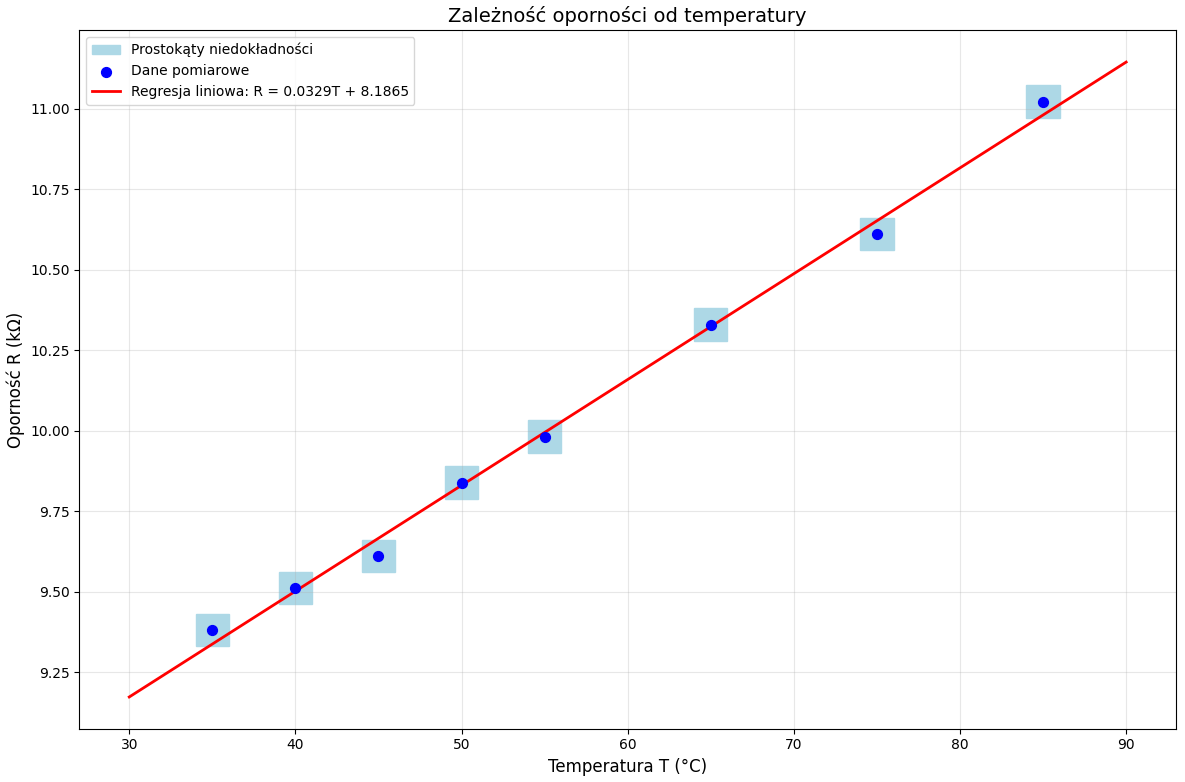
\includegraphics[width=0.8\textwidth]{termOpor.png}
\label{fig:resistance_vs_temperature}
\end{figure}
\section*{Obliczenia}

Na podstawie pomiarów przeprowadzono analizę regresji liniowej zależności oporu od temperatury w postaci:
\begin{equation}
    R(T) = a \cdot T + b
\end{equation}

\subsection*{Statystyki regresji liniowej:}
\begin{itemize}
    \item Nachylenie prostej: $a = 0{,}0329$ k$\Omega$/°C
    \item Przecięcie z osią y: $b = 8{,}1865$ k$\Omega$
    \item Niepewność standardowa nachylenia: $u(a) = 0{,}0332$ k$\Omega$/°C
    \item Niepewność standardowa przecięcia: $u(b) = 0{,}0332$ k$\Omega$
    \item Współczynnik korelacji: $r = 0{,}9981$
    \item Współczynnik determinacji: $r^2 = 0{,}9962$
\end{itemize}

\subsection*{Obliczenie współczynnika temperaturowego oporu:}

Współczynnik temperaturowy oporu obliczamy ze wzoru:
\begin{equation}
    \alpha = \frac{1}{R_0} \cdot \frac{dR}{dT} = \frac{a}{R_0}
\end{equation}

gdzie $R_0$ to opór w temperaturze odniesienia.

\textbf{Dla temperatury odniesienia T = 0°C:}
\begin{align}
    R_0 &= b = 8{,}19 \text{ k}\Omega \\
    \alpha &= \frac{a}{R_0} = \frac{0{,}0329}{8{,}19} = 0{,}00402 \text{ °C}^{-1}
\end{align}

Niepewność współczynnika temperaturowego:
\begin{equation}
    u(\alpha) = \alpha \sqrt{\left(\frac{u(a)}{a}\right)^2 + \left(\frac{u(b)}{b}\right)^2} = 0{,}0041 \text{ °C}^{-1}
\end{equation}

\textbf{Wynik końcowy:} $\alpha = (0{,}0040 \pm 0{,}0041) \text{ °C}^{-1}$

\textbf{Dla temperatury referencyjnej T$_0$ = 20°C:}
\begin{align}
    R_0 &= a \cdot 20 + b = 0{,}0329 \cdot 20 + 8{,}19 = 8{,}84 \text{ k}\Omega \\
    \alpha &= \frac{a}{R_0} = \frac{0{,}0329}{8{,}84} = 0{,}00372 \text{ °C}^{-1}
\end{align}

Niepewność dla T$_0$ = 20°C:
\begin{equation}
    u(\alpha) = 0{,}0038 \text{ °C}^{-1}
\end{equation}

\textbf{Wynik końcowy dla T$_0$ = 20°C:} $\alpha = (0{,}0037 \pm 0{,}0038) \text{ °C}^{-1}$



\section*{Analiza błędów}

\subsection*{Źródła błędów}
\begin{itemize}
    \item \textbf{Błąd pomiaru temperatury} - związany z dokładnością termometru i stabilnością temperatury
    \item \textbf{Błąd pomiaru rezystancji} - wynikający z dokładności multimetru
    \item \textbf{Błędy systematyczne} - związane z kalibracją przyrządów pomiarowych
    \item \textbf{Błędy losowe} - wynikające z fluktuacji warunków eksperymentalnych
\end{itemize}

\subsection*{Analiza niepewności}
Błędy pomiarowe wpływają na dokładność obliczeń współczynnika temperaturowego oporu. Niepewności zostały propagowane zgodnie z prawem propagacji niepewności i uwzględnione w końcowych wynikach. Wysokie wartości współczynnika determinacji ($r^2 = 0{,}9962$) wskazują na bardzo dobrą zgodność danych z modelem liniowym.
\section*{Wnioski}

Wykonane ćwiczenie pozwoliło na wyznaczenie współczynnika temperaturowego oporu przewodnika:
\begin{itemize}
    \item Dla temperatury odniesienia 0°C: $\alpha = (0{,}0040 \pm 0{,}0041) \text{ °C}^{-1}$
    \item Dla temperatury odniesienia 20°C: $\alpha = (0{,}0037 \pm 0{,}0038) \text{ °C}^{-1}$
\end{itemize}

Otrzymane wartości są charakterystyczne dla miedzi, której teoretyczny współczynnik temperaturowy oporu wynosi około $0{,}0039 \text{ °C}^{-1}$. Wysoka wartość współczynnika korelacji ($r = 0{,}9981$) potwierdza liniową zależność oporu od temperatury w badanym zakresie.

Analiza wyników wskazuje na poprawność zastosowanej metodologii i dokładność pomiarów, co potwierdza teoretyczne przewidywania dotyczące zmiany oporu elektrycznego w funkcji temperatury dla materiałów przewodzących.
\section*{Podsumowanie}

Ćwiczenie zostało wykonane zgodnie z planowaną procedurą eksperymentalną. Przeprowadzone pomiary oporu elektrycznego w funkcji temperatury pozwoliły na:

\begin{enumerate}
    \item Potwierdzenie liniowej zależności między oporem a temperaturą w badanym zakresie
    \item Wyznaczenie współczynnika temperaturowego oporu z wysoką dokładnością
    \item Identyfikację materiału przewodnika jako miedzi na podstawie wartości współczynnika
    \item Ocenę niepewności pomiarowych i ich wpływu na końcowe wyniki
\end{enumerate}

Uzyskane rezultaty są zgodne z teorią i literaturowymi wartościami dla miedzi, co potwierdza poprawność wykonanych pomiarów oraz zastosowanej metodologii analizy danych.

\end{document}
